%!TEX root = ../thesis.tex

\chapter{System Overview}
\label{sec:system_overview}

The system consists of two major parts: The Infrastructure side gathering and controlling temperature and organisational data, and the Mobile App side offering an user interface to view and control his temperature data and residential information. See Figure~\ref{fig:systemoverview} for a graphical overview.

\begin{figure}[h]
\begin{center}
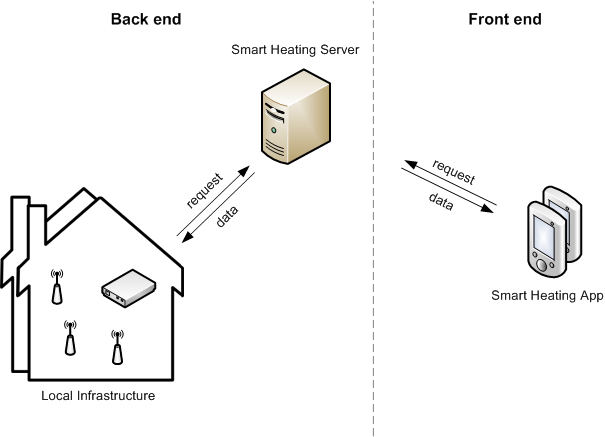
\includegraphics[width=0.8\textwidth]{images/SystemOverview.png}
\end{center}
\caption{System Overview}
\label{fig:systemoverview}
\end{figure}

The infrastructure part consists of a local residential part and a server part. Within the residence a small computer system is installed which serves as a proxy to the distributed low-power thermostats.
Whereas the server is the central entity to collect and store the accumulated sensor data and organizational data. Both parts are explained in the following chapters \ref{sec:infrastructure}~\nameref{sec:infrastructure} and \ref{sec:mobile_app}~\nameref{sec:mobile_app}.

\\

\section{Architecture}

The Smart Heating system is implemented using a server-client pattern. The Smart Heating Server provides an API which is consumed 


\section{Models}
\label{sec:system_overview_models}

Throughout the project there is a shared system model describing the underlying entities. The system model depicts the physical objects and places in the deployment that are used for data collection or organizational purposes. The following paragraphs describe the applied models and their associated design decisions.

\paragraph{Residence}

The fundamental unit of each deployment is the residence. Each residence corresponds to a installed local communication gateway. Further details are described in Section~\ref{sec:local_infrastructure}

\paragraph{User}

Each residence can contain multiple users. A user is associated to exactly one residence and is identified by its smart phone serial number. This design decision simplifies the system design and especially the user authentication, but also prevents a user from using the same identity when accessing the system from multiple smart phones.

\paragraph{Room and Thermostat}
A residence is divided in rooms where each room can contain several thermostats. A room is a simple organization approach to group multiple thermostats into a single unit.
%Eine Residence ist unterteilt in Räume wobei jeder Raum mehrere Thermostat enthalten kann.

\paragraph{Heating Table}

Each thermostat has an associated temperature schedule called heating table. The heating table is responsible for the assignment of each day and time in a week to a target temperature. The heating table is a periodic schedule repeating each week. This design decision was chosen for infrastructure simplicity as well as to reduce usability complexity.

\paragraph{Meta Entries}

Persist time depending meta information about thermostats. A meta entry consists of the received signal strength, up-time, battery level and an associated timestamp. This data can be used to identify issues regarding the thermostat devices such as wireless connection problems or drained batteries.